% =============================================================
%  Slide bao ve khoa luan tot nghiep
%  Title : Correlation-Aware Reward Exploration (CARE)
%  Author: Doan Van Giap - UET, VNU
%  Compile: pdflatex slides.tex (chay 2 lan de cap nhat label)
% =============================================================
\documentclass[10pt,aspectratio=169]{beamer}

% --- Font tieng Viet ---
\usepackage[utf8]{vietnam}
\usepackage[utf8]{inputenc}

% --- Math + Hinh ---
\usepackage{amsmath,amssymb,amsfonts,mathtools}
\usepackage{graphicx}
\usepackage{booktabs}
\usepackage{multirow}
\usepackage{array}
\usepackage{tikz}
\usetikzlibrary{calc,positioning,arrows.meta,fit,shapes}

% --- Theme ---
\usetheme{Madrid}
\usecolortheme{seahorse}
\useoutertheme{infolines}
\setbeamertemplate{navigation symbols}{}
\setbeamerfont{frametitle}{size=\large,series=\bfseries}
\setbeamerfont{title}{size=\Large,series=\bfseries}

% --- Mau nhan dien ---
\definecolor{uetblue}{RGB}{0, 51, 102}
\definecolor{uetorange}{RGB}{220, 110, 30}
\definecolor{softgray}{RGB}{120, 120, 120}
\definecolor{lightbg}{RGB}{245, 245, 240}

\setbeamercolor{title}{fg=uetblue}
\setbeamercolor{frametitle}{fg=uetblue}
\setbeamercolor{structure}{fg=uetblue}
\setbeamercolor{block title}{bg=uetblue,fg=white}
\setbeamercolor{block body}{bg=lightbg,fg=black}

\graphicspath{{../figures/}}

% --- Metadata ---
\title[CARE: Khám phá thích ứng theo trạng thái]{Nghiên cứu Động lực Nội tại trong Học Tăng cường}
\subtitle{Correlation-Aware Reward Exploration (CARE)}
\author[Đoàn Văn Giáp]{\textbf{Đoàn Văn Giáp}\\\footnotesize Giảng viên hướng dẫn: TS. Nguyễn Thị Thủy}
\institute[UET-VNU]{Trường Đại học Công nghệ - Đại học Quốc gia Hà Nội}
\date{Tháng 5, 2026}

\begin{document}

% =============================================================
% Slide 1 - Trang bia
% =============================================================
\begin{frame}[plain]
  \titlepage
  \begin{center}
    \footnotesize\color{softgray}
    Khóa luận tốt nghiệp -- Khoa Công nghệ Thông tin
  \end{center}
\end{frame}

% =============================================================
% Slide 2 - Boi canh va van de
% =============================================================
\begin{frame}{Bối cảnh: Bài toán phần thưởng thưa}
  \begin{columns}[T,onlytextwidth]
    \column{0.55\textwidth}
    \textbf{Học tăng cường (RL)} đã thành công với phần thưởng dày:
    \begin{itemize}\small
      \item Atari, AlphaGo, robot điều khiển
      \item Tác tử nhận tín hiệu thường xuyên $\Rightarrow$ dễ học
    \end{itemize}
    \vspace{0.3em}
    \textbf{Thực tế phần lớn bài toán là \textit{sparse reward}:}
    \begin{itemize}\small
      \item Tín hiệu chỉ xuất hiện sau chuỗi hành động dài
      \item Khám phá ngẫu nhiên gần như không bao giờ chạm đích
      \item Ví dụ: điều hướng, thao tác nhiều bước, mở khóa - lấy đồ
    \end{itemize}

    \column{0.42\textwidth}
    \begin{block}{Giải pháp phổ biến}
      \small Bổ sung \textbf{phần thưởng nội tại} $R^I$ (tò mò, độ mới) vào phần thưởng ngoại sinh $R^E$:
      \[
        \bar{r}_t \;=\; R^E_t \;+\; \beta\, R^{I,m}_t
      \]
      với $\beta$ là \textbf{hệ số cố định}.
    \end{block}
    \vspace{0.3em}
    \footnotesize\textcolor{softgray}{Các module nội tại tiêu biểu:\\ Count-based, ICM, RND, RIDE, RE3.}
  \end{columns}
\end{frame}

% =============================================================
% Slide 3 - Han che cua he so co dinh
% =============================================================
\begin{frame}{Hạn chế của hệ số $\beta$ cố định}
  \begin{block}{Vấn đề}
    Một $\beta$ \textit{duy nhất} áp dụng đồng đều cho \textit{mọi trạng thái} của môi trường.
  \end{block}

  \vspace{0.4em}
  \begin{columns}[T,onlytextwidth]
    \column{0.48\textwidth}
    \textbf{Nhu cầu khám phá phụ thuộc trạng thái:}
    \begin{itemize}\small
      \item Đầu episode, trước cửa chưa mở $\Rightarrow$ cần khám phá mạnh.
      \item Cuối episode, đã thấy đích $\Rightarrow$ cần khai thác, dập tò mò.
      \item $\beta$ cố định không phân biệt được hai loại trạng thái này.
    \end{itemize}

    \column{0.48\textwidth}
    \textbf{Ba bằng chứng kinh nghiệm:}
    \begin{itemize}\small
      \item $\beta$ tối ưu \textbf{khác nhau} giữa các môi trường (chênh tới 10$\times$).
      \item $\beta$ tối ưu \textbf{thay đổi theo giai đoạn} huấn luyện.
      \item $\beta$ \textbf{nhạy}: lệch một bậc giá trị có thể làm chính sách suy sụp ($\beta=0.05$ phá nát hầu hết môi trường trong thí nghiệm).
    \end{itemize}
  \end{columns}

  \vspace{0.4em}
  \begin{center}\itshape\small
    $\Rightarrow$ Cần một cơ chế \textbf{tự điều chỉnh $\beta$ theo từng trạng thái}, học trực tuyến từ chính kinh nghiệm của tác tử.
  \end{center}
\end{frame}

% =============================================================
% Slide 4 - Cau hoi nghien cuu & dong gop
% =============================================================
\begin{frame}{Câu hỏi nghiên cứu \& Đóng góp}
  \begin{block}{Câu hỏi nghiên cứu}
    \itshape Có thể học một hàm $\beta(s_t)$ \textbf{phụ thuộc trạng thái}, từ chính trải nghiệm tác tử, để cải thiện cách các module phần thưởng nội tại (count-based, ICM, RIDE) đóng góp vào việc học trong môi trường phần thưởng thưa hay không?
  \end{block}

  \vspace{0.4em}
  \textbf{Đóng góp chính:}
  \begin{enumerate}\small
    \item Đề xuất \textbf{CARE} -- Correlation-Aware Reward Exploration: một lớp \textit{scaling} thích ứng, học $\beta_\psi(s_t)$ qua \textbf{mục tiêu tương quan} với GAE advantage ngoại sinh.
    \item \textbf{Tính tổng quát theo module}: cùng cơ chế CARE áp dụng cho ba họ nội tại khác nhau (count-based, ICM, RIDE) -- không cần thiết kế lại.
    \item \textbf{Đánh giá thực nghiệm 570 lần chạy} trên 6 môi trường MiniGrid: CARE khớp hoặc vượt $\beta$ cố định tốt nhất ở \textbf{7/18 cặp (env, module)} mà không cần grid-search $\beta$.
  \end{enumerate}
\end{frame}

% =============================================================
% Slide 5 - Tong quan PPO + 3 module curiosity
% =============================================================
\begin{frame}{Nền tảng: PPO + 3 module phần thưởng nội tại}
  \begin{columns}[T,onlytextwidth]
    \column{0.42\textwidth}
    \textbf{PPO (Proximal Policy Optimization):}
    \begin{itemize}\small
      \item Actor--Critic, clipped surrogate
      \item GAE advantage ($\lambda=0.95$)
      \item $K=80$ epoch / 4{,}000 bước
    \end{itemize}
    \vspace{0.3em}
    \footnotesize Cùng backbone PPO cho mọi cấu hình $\Rightarrow$ so sánh \textbf{công bằng} giữa các module nội tại và các chiến lược scaling.

    \column{0.55\textwidth}
    \begin{block}{Ba module nội tại được khảo sát}
      \small
      \begin{tabular}{@{}p{1.2cm}p{6.0cm}@{}}
        \textbf{Count} & $R^I \propto 1/\sqrt{N(s)}$ qua random projection hash. \\[0.2em]
        \textbf{ICM}   & $R^I = \|\hat{\phi}(s') - \phi(s')\|^2$, lỗi dự báo của \textit{forward model} trong không gian embedding. \\[0.2em]
        \textbf{RIDE}  & $R^I = \|\phi(s')-\phi(s)\|_2 / \sqrt{N_\text{ep}(s')}$, "impact-driven" có giảm dần trong episode. \\
      \end{tabular}
    \end{block}
    \footnotesize\textcolor{softgray}{Mọi module đều được \textit{chuẩn hoá z-score} trước khi đưa vào CARE: $I^+ = \max(0, (R^I - \mu)/(\sigma+\varepsilon))$.}
  \end{columns}
\end{frame}

% =============================================================
% Slide 6 - CARE: Y tuong cot loi
% =============================================================
\begin{frame}{CARE -- Ý tưởng cốt lõi}
  \begin{block}{Thay đổi}
    Thay $\beta$ cố định bằng một mạng nhỏ $\beta_\psi(s_t)$ -- \textbf{Beta Network}.
    \[
      \bar{r}_t \;=\; R^E_t \;+\; \boxed{\beta_\psi(s_t)} \cdot I^{+}_t,
      \qquad \beta_\psi(s_t) \in [10^{-4},\, 5{\times}10^{-2}]
    \]
  \end{block}

  \begin{columns}[T,onlytextwidth]
    \column{0.5\textwidth}
    \textbf{Kiến trúc Beta Network:}
    \begin{itemize}\small
      \item Encoder 2 lớp (256) + đầu ra 128
      \item Sinh ra $\log \beta_\psi$, clip để $\beta \in [\beta_\text{min}, \beta_\text{max}]$
      \item Anchor $\beta_0 = \sqrt{\beta_\text{min}\,\beta_\text{max}} \approx 2.24{\times}10^{-3}$ (trung bình hình học = trung điểm log-space)
      \item Adam, lr $5{\times}10^{-4}$, 1 bước $\psi$/PPO update
    \end{itemize}

    \column{0.48\textwidth}
    \textbf{Tín hiệu giám sát: tương quan với extrinsic advantage.}\\[0.2em]
    Trực giác: \textit{khuếch đại tò mò ở những trạng thái mà chính sách đang vượt kỳ vọng giá trị; dập tò mò ở trạng thái còn lại.}
    \vspace{0.2em}
    \begin{center}
      \begin{tikzpicture}[node distance=0.4cm, font=\footnotesize]
        \node[draw,rounded corners,fill=lightbg,minimum width=2.0cm] (s) {state $s_t$};
        \node[draw,rounded corners,fill=uetblue!20,right=of s,minimum width=2.0cm] (b) {$\beta_\psi(s_t)$};
        \node[draw,rounded corners,fill=uetorange!20,below=of b,minimum width=2.0cm] (r) {$\bar{r}_t$};
        \draw[-{Latex[length=2mm]}] (s) -- (b);
        \draw[-{Latex[length=2mm]}] (b) -- (r);
        \node[below=0.05cm of r,font=\scriptsize\itshape,color=softgray] {(dùng trực tiếp, không Polyak target)};
      \end{tikzpicture}
    \end{center}
  \end{columns}
\end{frame}

% =============================================================
% Slide 7 - CARE: Cong thuc meta-loss
% =============================================================
\begin{frame}{CARE -- Mục tiêu huấn luyện $\beta_\psi$}
  \textbf{Meta-loss của Beta Network} (correlation + log-space regularizer):
  \[
    \mathcal{L}_\beta(\psi)
    \;=\;
    -\,\mathbb{E}\bigl[\,\hat{I}_z \cdot \hat{A}^E_z \,\bigr]
    \;+\;
    \lambda_\text{reg}\,\bigl(\log \beta_\psi(s) - \log \beta_0\bigr)^2
  \]
  \begin{itemize}\small
    \item $\hat{I} = \beta_\psi(s)\cdot I^+$ : phần thưởng nội tại đã có trọng số.
    \item $\hat{A}^E$ : GAE advantage ngoại sinh \textbf{thô}, chưa chuẩn hoá.
    \item $(\cdot)_z$ : z-score trong minibatch $\Rightarrow$ tương quan Pearson trong batch.
    \item $\lambda_\text{reg} = 10^{-3}$ : kéo $\beta_\psi$ về anchor $\beta_0$ khi không có tín hiệu.
  \end{itemize}
\end{frame}

% =============================================================
% Slide 8 - Sau moi truong MiniGrid
% =============================================================
\begin{frame}{6 môi trường MiniGrid}
  \centering
  \begin{tabular}{ccc}
    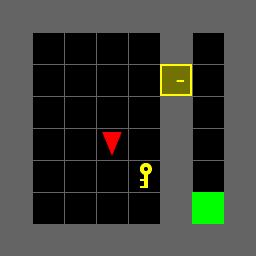
\includegraphics[height=2.6cm]{env_doorkey.png} &
    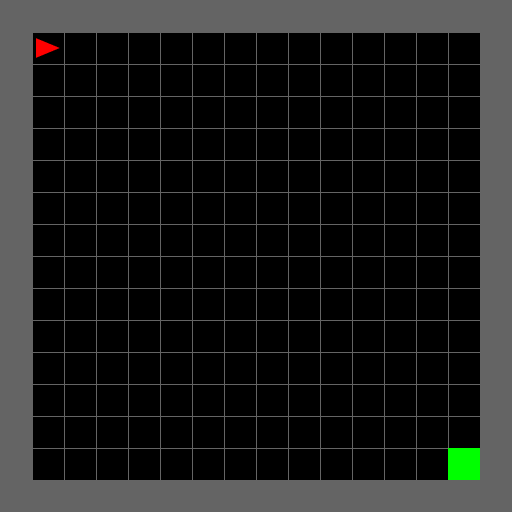
\includegraphics[height=2.6cm]{env_empty.png} &
    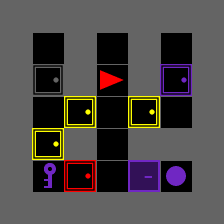
\includegraphics[height=2.6cm]{env_keycorridor.png} \\
    \scriptsize DoorKey-8x8 & \scriptsize Empty-16x16 & \scriptsize KeyCorridor-S3R3 \\[0.3em]
    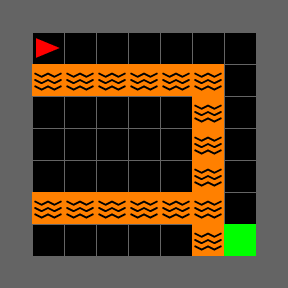
\includegraphics[height=2.6cm]{env_lavacrossing.png} &
    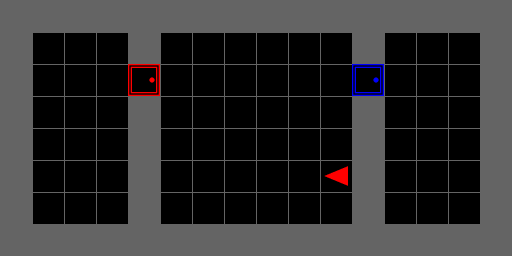
\includegraphics[height=2.6cm]{env_redbluedoors.png} &
    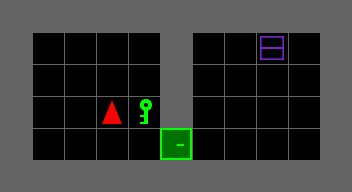
\includegraphics[height=2.6cm]{env_unlockpickup.png} \\
    \scriptsize LavaCrossing-S9N3 & \scriptsize RedBlueDoors-8x8 & \scriptsize UnlockPickup \\
  \end{tabular}

  \vspace{0.3em}
  \scriptsize\textcolor{softgray}{Tam giác đỏ: tác tử. Chìa vàng, cửa màu, ô lava, đích xanh khi có. Tất cả đều sparse-reward, grid rời rạc.}
\end{frame}

% =============================================================
% Slide 9 - Thiet ke thuc nghiem
% =============================================================
\begin{frame}{Thiết kế thực nghiệm}
  \begin{columns}[T,onlytextwidth]
    \column{0.5\textwidth}
    \textbf{6 môi trường MiniGrid:}
    \begin{itemize}\footnotesize
      \item DoorKey-8x8 -- chìa $\to$ cửa $\to$ đích
      \item Empty-16x16 -- thưởng cực thưa
      \item KeyCorridor-S3R3 -- nhiều phòng, nhiều chìa
      \item LavaCrossing-S9N3 -- né lava
      \item RedBlueDoors-8x8 -- thứ tự cửa
      \item UnlockPickup -- mở khóa rồi nhặt đồ
    \end{itemize}

    \column{0.48\textwidth}
    \textbf{19 cấu hình $\times$ 5 seeds $\times$ 6 envs = 570 lần chạy:}
    \begin{itemize}\footnotesize
      \item $B_0$: PPO không nội tại (kiểm soát)
      \item $F_{m,\beta}$: 3 module $\times$ 5 giá trị $\beta$ cố định\\
            $\beta \in \{0.0005, 0.001, 0.005, 0.01, 0.05\}$
      \item $C_m$: 3 biến thể CARE (count/ICM/RIDE)
    \end{itemize}
    \vspace{0.3em}
    \textbf{Mỗi seed: $10^6$ bước môi trường, $\sim$3--4 giờ trên T4 của Google Colab.}
  \end{columns}

  \vspace{0.3em}
  \begin{block}{Bốn chỉ số đánh giá}
    \footnotesize
    \begin{tabular}{@{}p{2.6cm}p{10.0cm}@{}}
      Episode return    & Phần thưởng trung bình của 10 episode cuối, lấy trung bình qua 5 seeds. \\
      Sample efficiency & Số bước đầu tiên đạt $0.7 \times$ phần thưởng cuối tốt nhất. \\
      Learning stability & Độ lệch chuẩn chéo seed của đường cong phần thưởng. \\
      Learned $\beta_\psi$ & Phân phối + heatmap theo vị trí tác tử. \\
    \end{tabular}
  \end{block}
\end{frame}

% =============================================================
% Slide 10a - Reward curves CARE-COUNT
% =============================================================
\begin{frame}{Đường cong phần thưởng: CARE-COUNT trên 6 môi trường}
  \centering
  
\includegraphics[width=0.95\linewidth,height=0.78\textheight,keepaspectratio]{all_envs_count.png}\\
  \scriptsize\textcolor{softgray}{Đường gạch (CARE-COUNT) so với 5 đường $\beta$ cố định (dải đỏ) và PPO không-nội-tại (xám). CARE-COUNT bám sát hoặc vượt $\beta$ cố định tốt nhất trên 4/6 env.}
\end{frame}

% =============================================================
% Slide 10b - Reward curves CARE-RIDE
% =============================================================
\begin{frame}{Đường cong phần thưởng: CARE-RIDE trên 6 môi trường}
  \centering
  
\includegraphics[width=0.95\linewidth,height=0.78\textheight,keepaspectratio]{all_envs_ride.png}\\
  \scriptsize\textcolor{softgray}{Đường gạch (CARE-RIDE) -- thắng rõ nhất trên \textbf{UnlockPickup} và \textbf{LavaCrossing} so với $\beta$ cố định tốt nhất.}
\end{frame}

% =============================================================
% Slide 10c - Reward curves CARE-ICM
% =============================================================
\begin{frame}{Đường cong phần thưởng: CARE-ICM trên 6 môi trường}
  \centering
  
\includegraphics[width=0.95\linewidth,height=0.78\textheight,keepaspectratio]{all_envs_icm.png}\\
  \scriptsize\textcolor{softgray}{Đường gạch (CARE-ICM) -- \textbf{sụp trên KeyCorridor (0.000)} và phương sai cao trên 3 env khác. ICM tín hiệu nhiễu $\Rightarrow$ CARE khuếch đại nhiễu.}
\end{frame}

% =============================================================
% Slide 10d - Tong hop: CARE-COUNT & CARE-RIDE khop hoac vuot
% =============================================================
\begin{frame}{Kết quả: CARE-COUNT \& CARE-RIDE -- khớp hoặc vượt}
  \begin{columns}[T,onlytextwidth]
    \column{0.55\textwidth}
    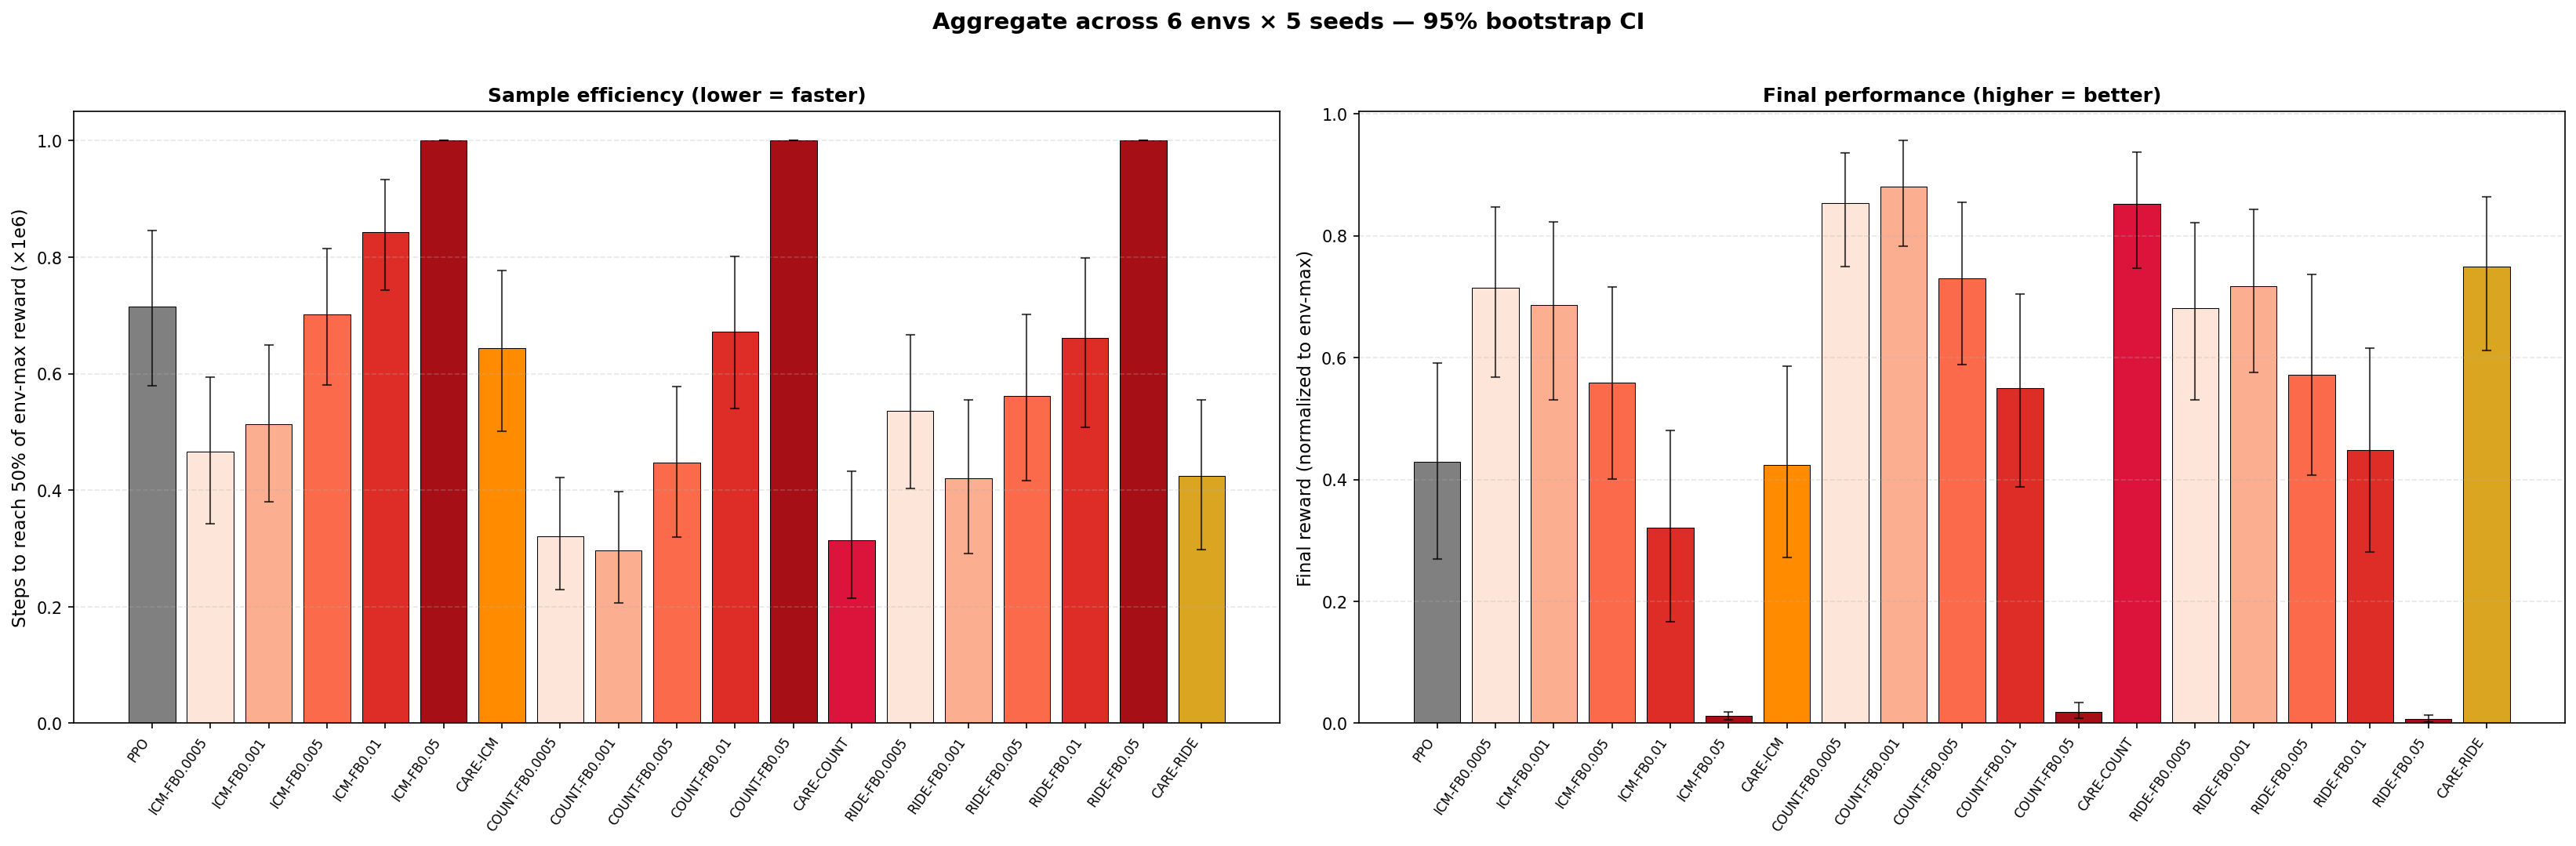
\includegraphics[width=\linewidth]{aggregate_summary.png}\\
    \footnotesize\textcolor{softgray}{Hình: Tổng hợp sample-efficiency (nhỏ tốt) và normalized final reward (lớn tốt) trên 6 môi trường.}

    \column{0.42\textwidth}
    \textbf{Tổng quan 18 cặp (env, module):}
    \begin{itemize}\footnotesize
      \item CARE \textbf{khớp hoặc vượt} $\beta$ cố định tốt nhất: \textbf{7/18} (gồm 3 vượt và 4 hoà $\pm 0.005$).
      \item Kém hơn: \textbf{11/18} (đa số ở ICM và RedBlueDoors).
    \end{itemize}
    \vspace{0.3em}
    \textbf{Điểm sáng:}
    \begin{itemize}\footnotesize
      \item \textbf{CARE-RIDE trên UnlockPickup}: $0.536$ vs $0.369$ \textit{(+0.167)}.
      \item \textbf{CARE-COUNT trên Empty-16x16}: chạm ngưỡng \textbf{66k bước} (vs 82k tốt nhất của $\beta$ cố định).
      \item Phương sai thấp nhất trên mọi env mà CARE-COUNT hội tụ.
    \end{itemize}
  \end{columns}
\end{frame}

% =============================================================
% Slide 11 - Ket qua 2: beta(s) hoc duoc
% =============================================================
\begin{frame}{Kết quả: $\beta_\psi(s)$ thật sự phụ thuộc trạng thái}
  \begin{columns}[T,onlytextwidth]
    \column{0.5\textwidth}
    \centering
    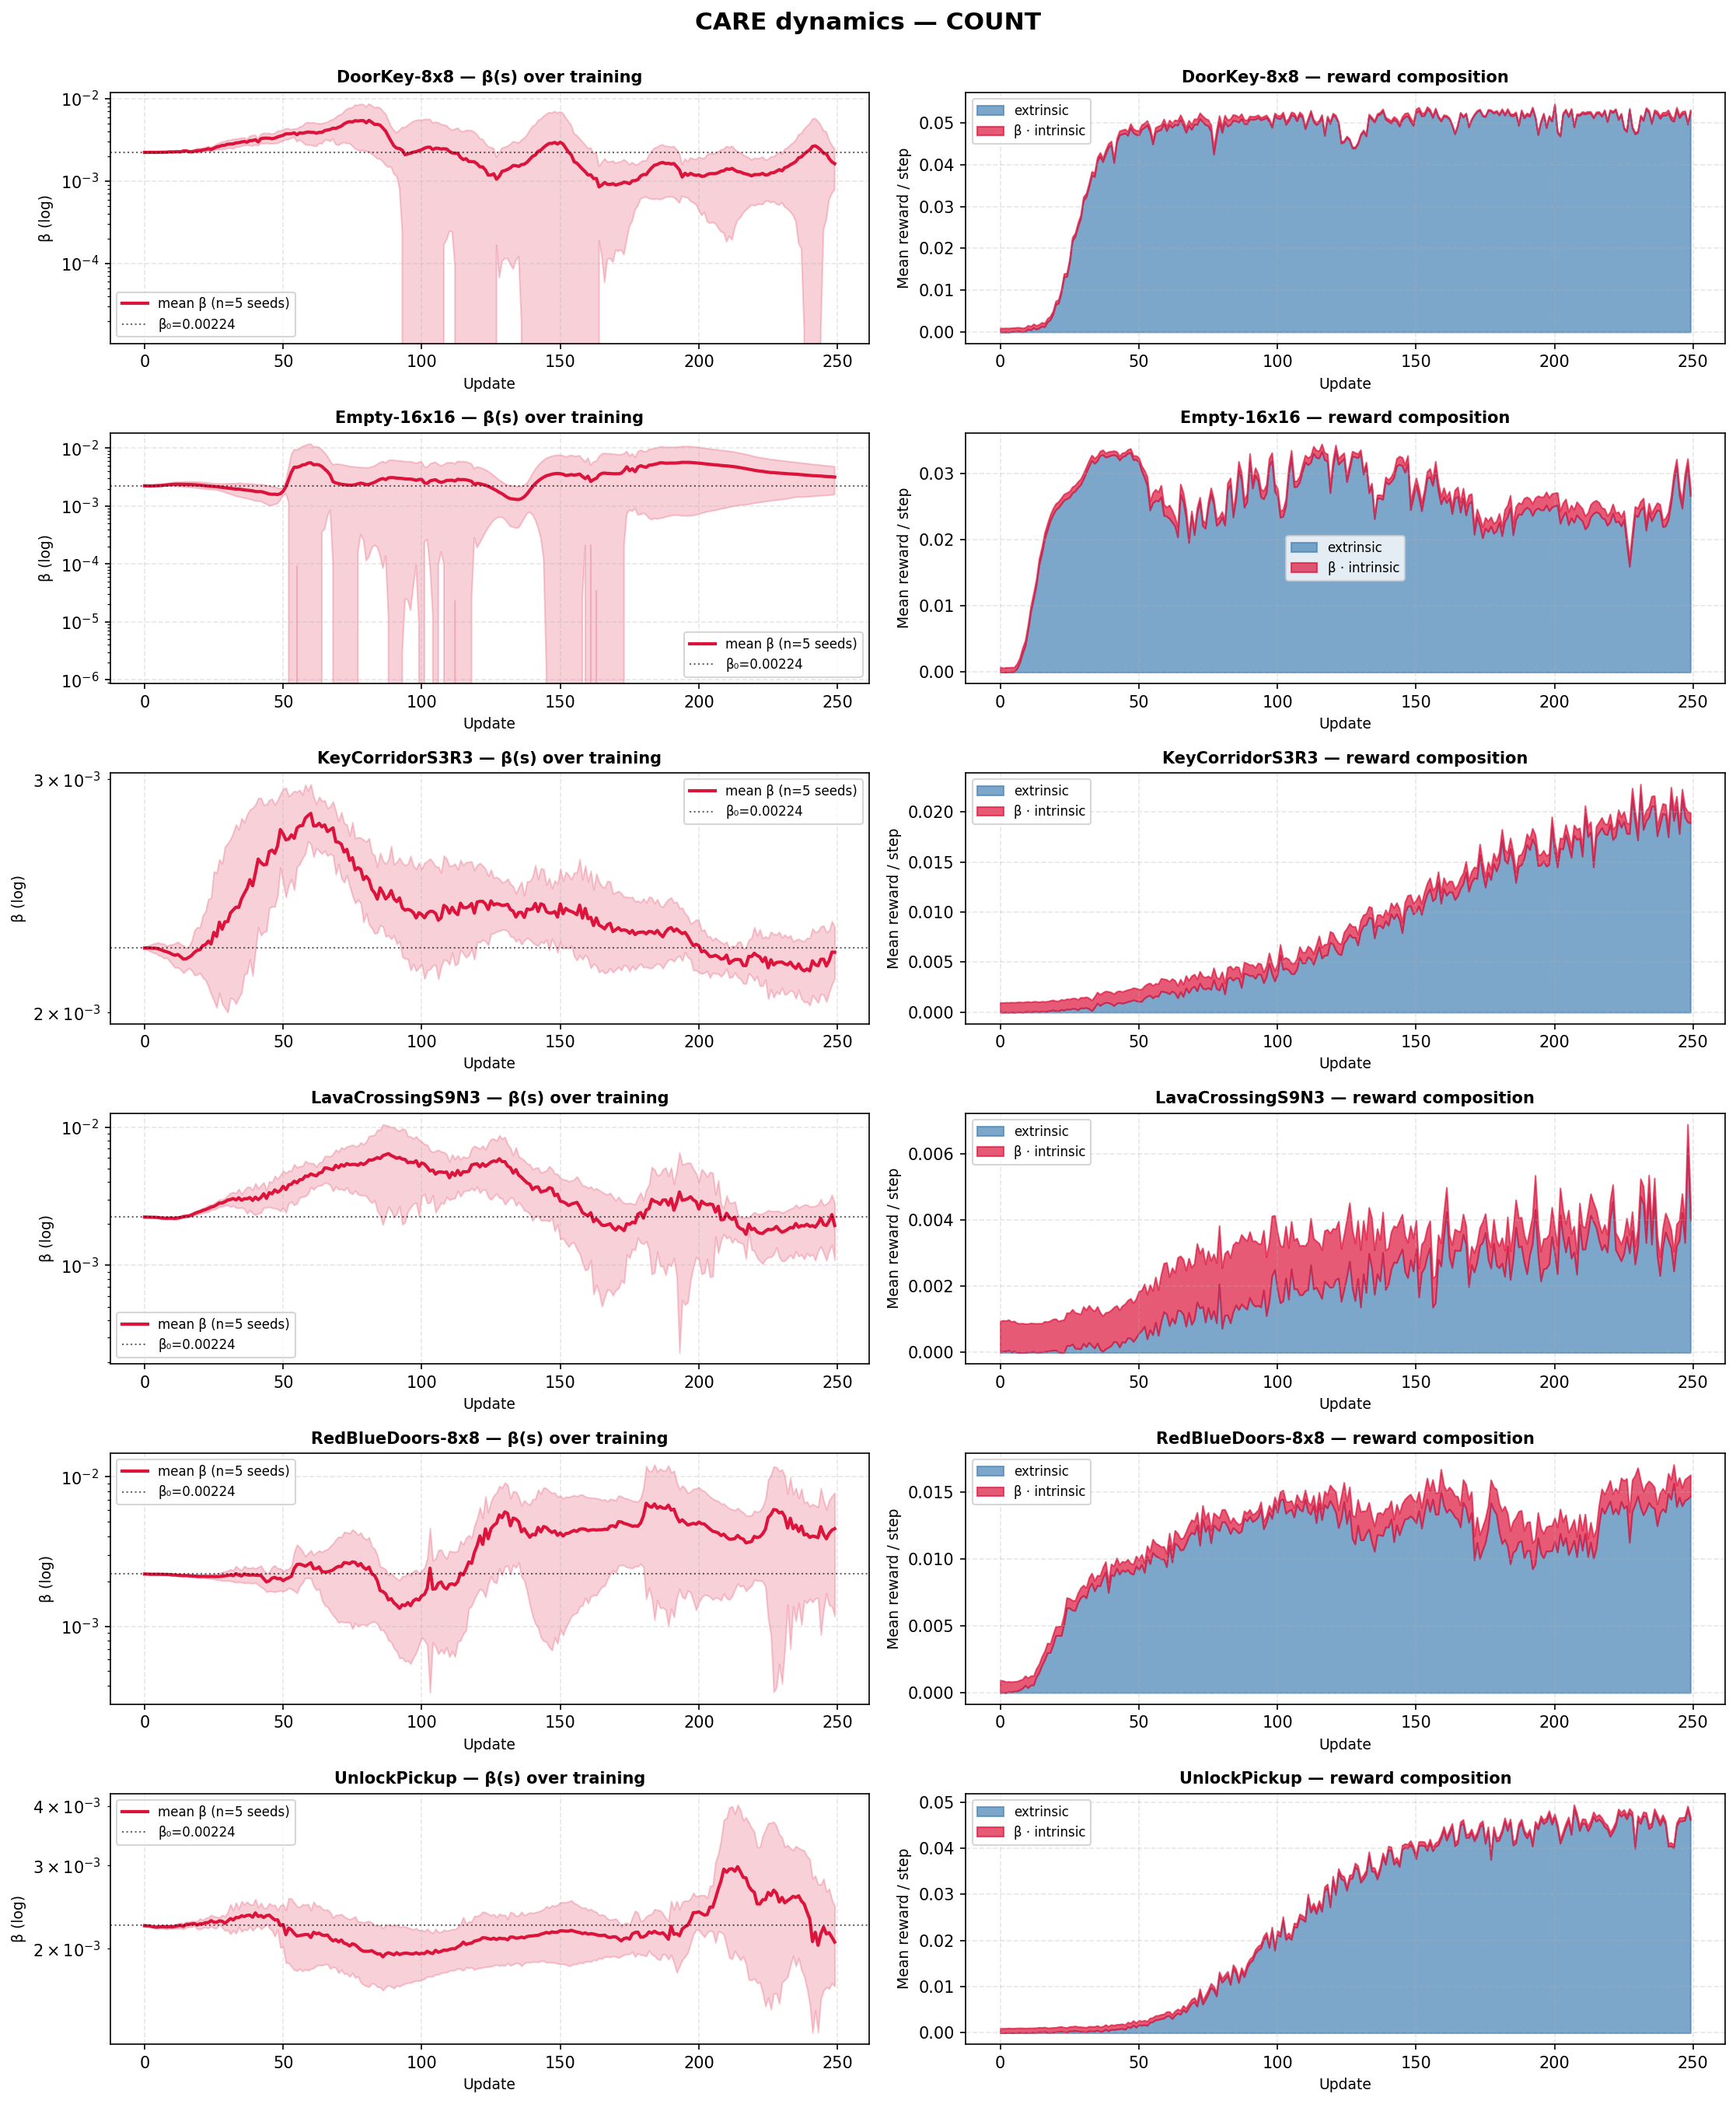
\includegraphics[width=\linewidth,height=0.45\textheight,keepaspectratio]{care_dynamics_count.png}\\
    \scriptsize\textcolor{softgray}{CARE-COUNT: mean $\beta_\psi(s_t)$ qua thời gian.}

    \column{0.5\textwidth}
    \centering
    
\includegraphics[width=\linewidth,height=0.45\textheight,keepaspectratio]{care_beta_hist_ride.png}\\
    \scriptsize\textcolor{softgray}{CARE-RIDE: histogram $\beta_\psi$ cuối training.}
  \end{columns}
  \vspace{0.3em}
  \textbf{\small Ba chế độ quan sát được:}
  \begin{enumerate}\scriptsize
    \item \textbf{Extrinsic sớm} (DoorKey, Empty): $\beta_\psi$ tách khỏi $\beta_0$ trong $\sim 10$ update đầu, giảm về $\beta_\text{min}$.
    \item \textbf{Extrinsic giữa training} (KeyCorridor, RedBlueDoors, UnlockPickup): $\beta_\psi$ \textit{neo tại $\beta_0$} ở giai đoạn cold-start, chỉ tách khi advantage có độ lớn đáng kể.
    \item \textbf{Phân phối cuối $\beta_\psi$ trải $\sim$1 bậc giá trị} qua các trạng thái -- bằng chứng học được hàm \textit{thật sự phụ thuộc trạng thái}, không suy biến về một hằng.
  \end{enumerate}
\end{frame}

% =============================================================
% Slide 12 - Phan tich that bai: CARE-ICM
% =============================================================
\begin{frame}{Phân tích thất bại: vì sao CARE-ICM kém?}
  \begin{columns}[T,onlytextwidth]
    \column{0.46\textwidth}
    \centering
    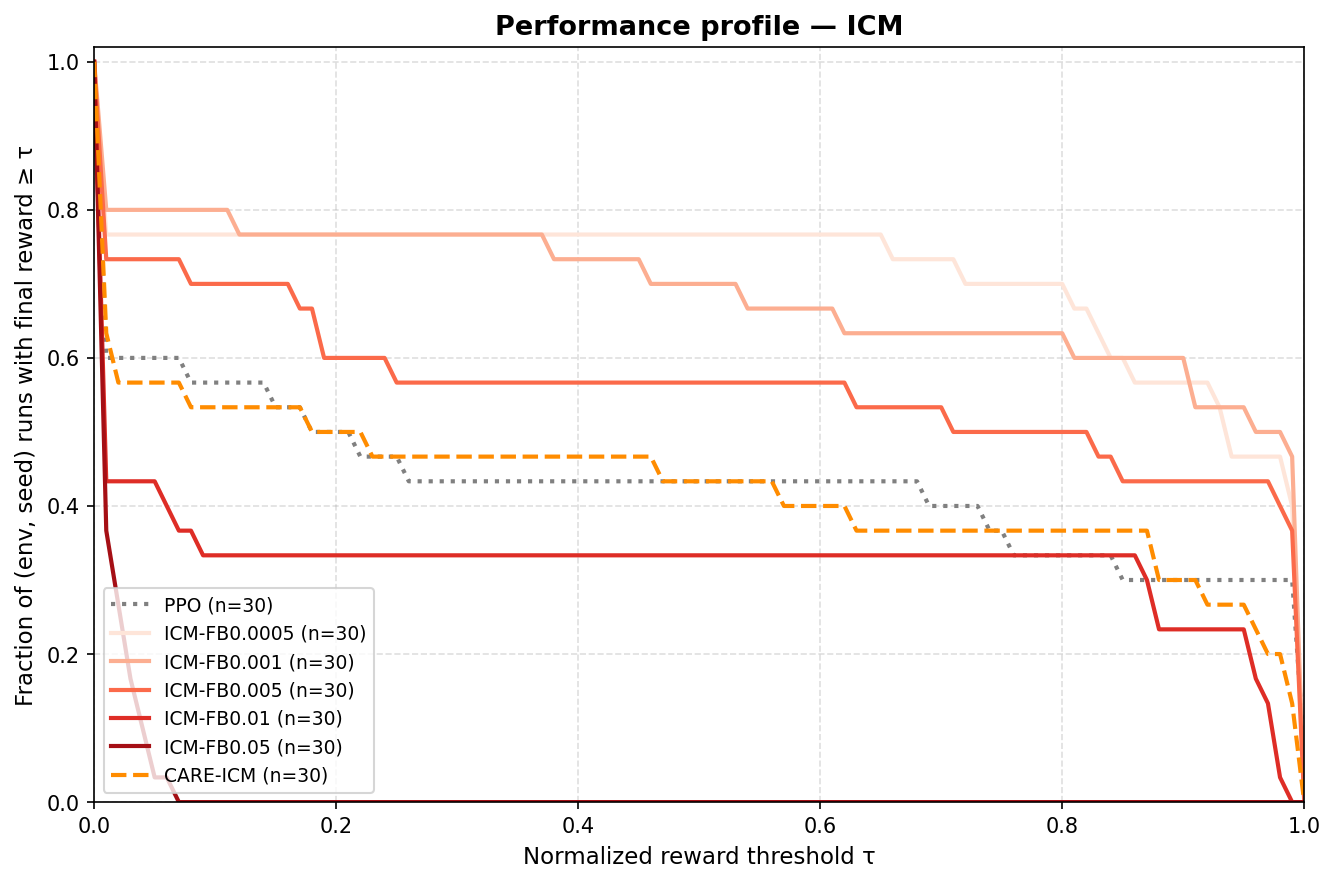
\includegraphics[width=\linewidth]{profile_icm.png}\\
    \footnotesize\textcolor{softgray}{Performance profile cho module ICM -- CARE bị nhiều $\beta$ cố định nhỏ vượt.}

    \column{0.5\textwidth}
    \textbf{Trường hợp tiêu biểu: KeyCorridor.}
    \begin{itemize}\footnotesize
      \item Best fixed-$\beta$ (ICM, $\beta{=}0.001$): $0.457$.
      \item CARE-ICM: \textbf{0.000} (cả 5 seed).
    \end{itemize}
    \vspace{0.3em}
    \textbf{Cơ chế thất bại:}
    \begin{itemize}\footnotesize
      \item Lỗi forward-model ICM \textit{không nhất thiết} nằm trên đường tới đích.
      \item Vùng có $I^+$ lớn \textbf{nhưng advantage cũng dương ngẫu nhiên} $\Rightarrow$ cov dương \textit{nhầm}.
      \item Gradient $\mathcal{L}_\beta$ \textbf{khuếch đại} $\beta_\psi$ ở vùng \textit{ngoài} đường tới đích.
      \item Histogram CARE-ICM trên KeyCorridor: \textbf{bimodal, đuôi nặng gần $\beta_\text{max}$}.
    \end{itemize}
  \end{columns}

  \vspace{0.3em}
  \begin{block}{Bài học}
    \footnotesize CARE \textbf{không phải} thay thế cho việc chọn module nội tại tốt. Đó là một bộ nhân phụ thuộc trạng thái mà chất lượng phụ thuộc vào \textit{độ tương quan} giữa tín hiệu nội tại thô và đường tới đích (extrinsic-success path).
  \end{block}
\end{frame}

% =============================================================
% Slide 13 - Ket luan & gioi han
% =============================================================
\begin{frame}{Kết luận \& Giới hạn}
  \textbf{Đóng góp đã được kiểm chứng:}
  \begin{itemize}\small
    \item Một cơ chế \textbf{scaling thích ứng theo trạng thái} cho phần thưởng nội tại, được huấn luyện qua mục tiêu \textbf{tương quan với GAE advantage}.
    \item Cùng cơ chế CARE \textbf{áp dụng được cho 3 họ module}, không cần thiết kế lại.
    \item Trên \textbf{count-based và RIDE}: CARE khớp/vượt $\beta$ cố định tốt nhất \textit{không cần} grid-search.
  \end{itemize}

  \vspace{0.3em}
  \textbf{Giới hạn:}
  \begin{itemize}\small
    \item \textbf{Phụ thuộc chất lượng module}: CARE \textbf{không cứu được ICM} khi tín hiệu thô không khớp đường-tới-đích (KeyCorridor: 0.000).
    \item \textbf{Cold-start trên môi trường cực thưa} (Empty-16x16): advantage gần như 0 ở mọi trạng thái, gradient của correlation gần như nhiễu, $\beta_\psi$ rớt về $\beta_0$ -- CARE \textit{thoái biến về fixed-$\beta$}.
    \item \textbf{Phạm vi MiniGrid}: action rời rạc, observation thấp chiều. Chưa kiểm chứng trên continuous control hoặc môi trường giàu observation.
  \end{itemize}
\end{frame}

% =============================================================
% Slide 14 - Huong phat trien & Q&A
% =============================================================
\begin{frame}{Hướng phát triển \& Câu hỏi}
  \textbf{Hướng mở rộng:}
  \begin{enumerate}\small
    \item \textbf{Mở rộng phạm vi}: continuous control (MuJoCo, robotic manipulation), multi-task RL, embodied navigation.
    \item \textbf{Phân tích lý thuyết sâu hơn} cho mục tiêu tương quan -- khi nào adaptive scaling chắc chắn có lợi?
    \item \textbf{Tín hiệu giám sát thay thế}: bootstrapped novelty, trajectory-level success indicator -- khắc phục regime cold-start cực thưa.
    \item \textbf{Lai ghép}: CARE + meta-gradient method, hoặc CARE + diversity-based exploration.
  \end{enumerate}

  \vspace{1em}
  \begin{center}
    {\Huge\bfseries\color{uetblue} Xin cảm ơn Hội đồng!}\\[0.5em]
    \footnotesize\textcolor{softgray}{Đoàn Văn Giáp -- juuzou152@gmail.com}
  \end{center}
\end{frame}

% =============================================================
% Backup slides (khong tinh vao 14 slide chinh)
% =============================================================
\appendix

\begin{frame}{[Backup] Bảng đối sánh CARE vs best fixed-$\beta$ (18/18)}
  \centering\scriptsize
  \begin{tabular}{|l|l|c|c|c|c|}
    \hline
    \textbf{Env} & \textbf{Module} & \textbf{CARE} & \textbf{Best fixed} & \textbf{Best $\beta$} & \textbf{Gap} \\
    \hline
    \multirow{3}{*}{DoorKey-8x8} & COUNT & 0.973 & 0.973 & 0.0005 & \textbf{+0.001} \\
     & ICM   & 0.770 & 0.973 & 0.0005 & -0.202 \\
     & RIDE  & 0.973 & 0.973 & 0.0005 & \textbf{+0.000} \\
    \hline
    \multirow{3}{*}{Empty-16x16} & COUNT & 0.959 & 0.975 & 0.0005 & -0.017 \\
     & ICM   & 0.575 & 0.975 & 0.0005 & -0.400 \\
     & RIDE  & 0.941 & 0.974 & 0.001  & -0.033 \\
    \hline
    \multirow{3}{*}{KeyCorridor} & COUNT & 0.831 & 0.828 & 0.001 & \textbf{+0.003} \\
     & ICM   & 0.000 & 0.457 & 0.001 & -0.457 \\
     & RIDE  & 0.548 & 0.703 & 0.001 & -0.155 \\
    \hline
    \multirow{3}{*}{LavaCrossing} & COUNT & 0.372 & 0.530 & 0.001 & -0.158 \\
     & ICM   & 0.077 & 0.060 & 0.001 & \textbf{+0.017} \\
     & RIDE  & 0.543 & 0.512 & 0.0005 & \textbf{+0.031} \\
    \hline
    \multirow{3}{*}{RedBlueDoors} & COUNT & 0.653 & 0.779 & 0.0005 & -0.126 \\
     & ICM   & 0.273 & 0.737 & 0.0005 & -0.464 \\
     & RIDE  & 0.593 & 0.794 & 0.001  & -0.201 \\
    \hline
    \multirow{3}{*}{UnlockPickup} & COUNT & 0.936 & 0.936 & 0.0005 & \textbf{+0.000} \\
     & ICM   & 0.716 & 0.937 & 0.001 & -0.221 \\
     & RIDE  & \textbf{0.536} & 0.369 & 0.0005 & \textbf{+0.167} \\
    \hline
  \end{tabular}
\end{frame}

\begin{frame}{[Backup] Pseudocode CARE (Algorithm 1)}
  \footnotesize
  \begin{enumerate}
    \item Khởi tạo $\pi_\theta$, $V_\phi$, Beta Network $\beta_\psi$, intrinsic module $m$.
    \item \textbf{Lặp} đến $T$ bước:
    \begin{enumerate}\footnotesize
      \item Thu thập rollout $\{(s_t,a_t,r^E_t,s_{t+1})\}$ với $\pi_\theta$.
      \item Tính $R^{I,m}_t$ từ module $m$; chuẩn hoá $I^+_t$.
      \item Tính $\beta_\psi(s_t)$ và shaped reward $\bar{r}_t = r^E_t + \beta_\psi(s_t)\cdot I^+_t$.
      \item Tính GAE advantage $\hat{A}^E_t$ \textbf{thô} (từ extrinsic) và $\hat{A}^{\text{shaped}}_t$ (cho policy).
      \item Cập nhật $\pi_\theta$, $V_\phi$ bằng PPO ($K{=}80$ epoch, $\hat{A}$ chuẩn hoá).
      \item \textbf{Một bước} Adam trên $\psi$: $\mathcal{L}_\beta = -\mathbb{E}[\hat{I}_z\,\hat{A}^E_z] + \lambda_\text{reg}(\log\beta_\psi - \log\beta_0)^2$.
      \item Clip $\beta_\psi$ vào $[\beta_\text{min},\beta_\text{max}]$.
    \end{enumerate}
  \end{enumerate}
\end{frame}

\begin{frame}{[Backup] Hyperparameter chính}
  \footnotesize
  \begin{tabular}{ll}
    \toprule
    \textbf{PPO} & $K=80$, $\epsilon_\text{clip}=0.2$, $\gamma=0.99$, $\lambda_\text{GAE}=0.95$ \\
                 & lr$_\text{actor}=3{\times}10^{-4}$, lr$_\text{critic}=10^{-3}$, rollout $T=4{,}000$ \\
    \midrule
    \textbf{CARE} & $\beta_\text{min}=10^{-4}$, $\beta_\text{max}=5{\times}10^{-2}$ \\
                  & $\beta_0=\sqrt{\beta_\text{min}\beta_\text{max}}\approx 2.24{\times}10^{-3}$ \\
                  & $\lambda_\text{reg}=10^{-3}$, lr$_\psi=5{\times}10^{-4}$, weight-decay $10^{-6}$ \\
                  & 1 bước $\psi$/PPO update, grad-clip L2 $1.0$, không Polyak target \\
    \midrule
    \textbf{Sweep $\beta$ cố định} & $\beta \in \{0.0005,\,0.001,\,0.005,\,0.01,\,0.05\}$ \\
    \midrule
    \textbf{Seeds} & $\{1,2,3,4,5\}$, mỗi run $10^6$ bước \\
    \bottomrule
  \end{tabular}
\end{frame}

\end{document}
